%\documentclass[10pt,twocolumn,letterpaper,draft]{article}
\documentclass[10pt,letterpaper]{ctexart}

\usepackage{cvpr}
% \usepackage{epsfig}
\usepackage{graphicx}
\usepackage{amsmath}
\usepackage{amssymb}
\usepackage{booktabs}
\usepackage{subfigure}
\usepackage{algorithm}
\usepackage{algorithmicx}
\usepackage{algpseudocode}
\usepackage{listings}

\lstset{language=C++,
    basicstyle=\ttfamily,
    frame=single,
    keywordstyle=\color{blue}\ttfamily,
    stringstyle=\color{magenta}\ttfamily,
    commentstyle=\color{green}\ttfamily,
    morecomment=[l][\color{magenta}]{\#},
    morekeywords={*,uint_fast64_t}
}

\renewcommand{\labelenumi}{\alph{enumi}.} % Make numbering in the enumerate environment by letter rather than number (e.g. section 6)
\floatname{algorithm}{算法}
\renewcommand{\algorithmicrequire}{\textbf{输入:}}
\renewcommand{\algorithmicensure}{\textbf{输出:}}
\renewcommand{\lstlistingname}{代码清单}

\usepackage{enumitem}
\setenumerate[1]{itemsep=0pt,partopsep=0pt,parsep=\parskip,topsep=5pt}
\setitemize[1]{itemsep=0pt,partopsep=0pt,parsep=\parskip,topsep=5pt}
\setdescription{itemsep=0pt,partopsep=0pt,parsep=\parskip,topsep=5pt}

% Include other packages here, before hyperref.

% If you comment hyperref and then uncomment it, you should delete
% egpaper.aux before re-running latex.  (Or just hit 'q' on the first latex
% run, let it finish, and you should be clear).
\usepackage[pagebackref=true,breaklinks=true,letterpaper=true,colorlinks,bookmarks=false]{hyperref}


\cvprfinalcopy % *** Uncomment this line for the final submission

\def\cvprPaperID{159} % *** Enter the CVPR Paper ID here
\def\httilde{\mbox{\tt\raisebox{-.5ex}{\symbol{126}}}}

\newcommand{\mypara}[1]{\paragraph{#1.}}

\graphicspath{{figures/}}

% Pages are numbered in submission mode, and unnumbered in camera-ready
%\ifcvprfinal\pagestyle{empty}\fi
\setcounter{page}{1}


%\begin{CJK*}{GBK}{song}

\newcommand{\figref}[1]{图\ref{#1}}
\newcommand{\tabref}[1]{表\ref{#1}}
\newcommand{\equref}[1]{式\ref{#1}}
\newcommand{\secref}[1]{第\ref{#1}节}

\ctexset{
  section={
          name={,、},
          number={\chinese{section}},
          format={\heiti},
          beforeskip={0.1ex},
          afterskip={0.1ex},
          aftername={\nobreak},
          indent={\parindent},
          },
}
\usepackage{zhnumber}

\newcommand\zhsubsec[1]{{% 中文小节
\bfseries{
\stepcounter{subsection}(\zhnum{subsection}){#1}}
\vspace{0.1pt}%
}}

%%%%%%%%% TITLE
\begin{document}
\pagestyle{plain}
\title{
    \begin{center}
        \phantom{Start!}
        \vspace{2cm}
        \center{\zihao{1} 中山大学数据科学与计算机学院}
        \center{\zihao{2} 《高性能程序设计基础》实验6}
        \center{(2018-2019学年秋季学期)}
    \end{center}
}
\maketitle

\begin{center}
    \setlength{\baselineskip}{40pt}
    \vspace{1cm}
    \zihao{-2}
    \center{
        \begin{tabular}{cc}
        学\qquad 号:& \underline{~~~~~~16337113~~~~~~}  \\
        姓\qquad 名:& \underline{~~~~~~~劳马东~~~~~~~}  \\
        教学班级:   & \underline{~~~~~教务2班~~~~~}  \\
        专\qquad 业:& \underline{~~~~~~~~~超算~~~~~~~~}  \\
       \end{tabular}
    }
\end{center}
\pagebreak

%%%%%%%%% BODY TEXT %%%%%%%%%%%%
% \begin{enumerate}[itemindent=2.5em,label=\arabic*、]
% \end{enumerate}

% \begin{algorithm}
%     \begin{algorithmic}[1] %每行显示行号
%         \Function {$TreeSearch$}{$Frontier, Successors,
%         \EndFunction
%     \end{algorithmic}
% \end{algorithm}

% \begin{figure}[h]
%   \centering
%   \subfigure[Completeness]{
%   \includegraphics[width=0.4\textwidth]{dfs-1.png}
%   \label{fig:dfs-1}}
% \end{figure}

\section{实验题目}
\begin{enumerate}[itemindent=1.5em,label=\arabic*、]
\item 完成正则采样排序PSRS的MPI算法;
\item 按要求使用MPI集合通信。
\end{enumerate}

\section{正则采样排序概述}
快速排序算法的效率相对较高,并行算法在理想的情况下时间复杂度可达到$O(n)$,但它有一个严重的问题:
会造成严重的负载不平衡,最差情况下算法的复杂度可达$O(n^2)$。并行正则采样排序克服了这一缺点,
是一种基于均匀划分的负载平衡的并行排序算法。

\zhsubsec{算法流程}

\begin{figure}[H]
  \centering
  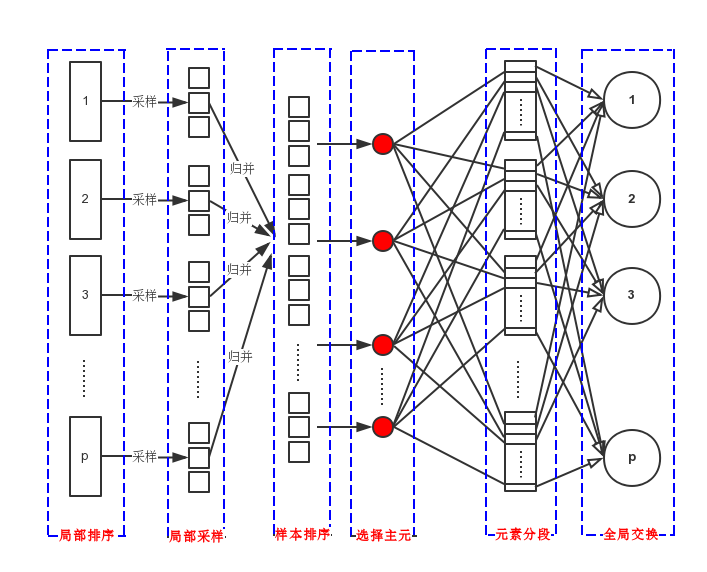
\includegraphics[width=0.7\textwidth]{steps.png}
  \label{fig:steps}
  \caption{正则采样排序示意图}
\end{figure}

\par 假设待排序的元素n个,处理器p个,算法大体流程如下。
\begin{enumerate}[itemindent=3em,label=\arabic*、]
  \item 首先将这n个元素均匀的分成p部分,每部分包含$\frac{n}{p}$个元素(如图1矩形)。每个处理器负责其中的一部分,并对其进行局部排序;
  \item 为确定局部有序序列在整个序列中的位置,每个处理器从各自的局部有序序列中选取几个代表元素(如图1第一列正方形);
  \item 将这些代表元素进行排序后选出p-1个主元(如图1红色圆形);
  \item 每个处理器根据这p-1个主元将自己的局部有序序列分成p段;
  \item 然后通过全局交换的方式,将p段有序序列分发给对应的处理器(如图1大圆),使第i个处理器都拥有各个处理器的第i段,
  共p段有序序列。
  \item 每个处理器对这p段有序序列进行排序。最后,将各个处理器的有序段按顺序汇合起来,就是全局有序序列了。
\end{enumerate}

\section{实验过程}
\zhsubsec{元素划分与采样}

出于方便和性能考虑,每个进程直接从文件中并行读取元素。并行读取最重要的是解决文件指针
定位的问题,即每个进程该从什么位置开始读取多少个元素?假设$p$个进程分别编号为$0、1...p-2、p-1$,
则显然进程$i$开始读的位置是前$i-1$个进程所读元素的和,即:
\begin{equation}
  f(i) =
    \begin{cases}
      f(i-1) + balance(i-1) & i=1, 2, ..., p-2, p-1\\
      0 & i=0
    \end{cases}
\end{equation}
其中$balance$函数返回对应进程的负载,即读取多少个元素。
\par 那么如何相对均衡地分配负载呢?方法是先给每个进程分配$\lfloor\frac{n}{p}\rfloor$
个元素,然后将剩下的$r$个元素分配给编号$0$到$r-1$的进程。
\begin{lstlisting}[caption=并行读取元素,label={code:read},captionpos=b]
vector<uint_fast64_t> divide_read_directly(istream& in, 
                                            uint_fast64_t n, 
                                            MPI_Comm comm) 
{
    Comm_Info info(comm);
    // 获取每个进程对应的负载(均衡)
    vector<uint_fast64_t> balance = get_v<uint_fast64_t>(n, info.comm_size);
    // 得到自己的负载的元素个数
    uint_fast64_t my_balance = balance[info.rank];
    vector<uint_fast64_t> local(my_balance);
    // 计算负载的前缀和,每个数代表对应进程开始读的位置
    vector<uint_fast64_t> prefixes = get_prefix_sum<uint_fast64_t>(balance);
    // 每个数8个字节,指针定位时乘上8(加1是为了跳过开头表示元素总数的那个数)
    in.seekg((prefixes[info.rank] + 1) * 8, ios::beg);
    for (auto& x: local)
        read(in, x);
    return local;
}
\end{lstlisting}

\begin{enumerate}[itemindent=2.5em,label=\arabic*、]
\item 本地数据排序
\par \qquad 排序原则上采用任何排序算法都可以,但是由于数据量比较大,如果使用空间复杂度
较大的算法(如快速排序和归并排序),就很容易超出内存限制,导致程序崩溃。因此,实验中使用
了STL的堆排序算法,时间复杂度是$O(n \log n)$,空间复杂度是$O(1)$。
\item 按进程数p等间隔采样
\par \qquad 每个进程从其局部有序序列中选取$p$个样本,因此总共有$p^2$个样本,取数间隔为$\frac{n}{p^2}$。
\begin{lstlisting}[caption=排序与采样,label={code:local_sample},captionpos=b]
make_heap(local.begin(), local.end());
sort_heap(local.begin(), local.end());
  
int num_samples = info.comm_size * info.comm_size;
vector<uint_fast64_t> sample = copy_every_n(local, n / num_samples);
\end{lstlisting}

\end{enumerate}

\zhsubsec{划分主元}
\begin{enumerate}[itemindent=2.5em,label=\arabic*、]
\item 收集样本:一个进程(0号)用MPI\_Gatherv收集样本并对所有样本进行排序;
\item 采样获得主元:按进程数p对全体样本等间隔采样;
\item 用MPI\_Bcast广播主元。
\end{enumerate}

\begin{lstlisting}[caption=划分主元并广播,captionpos=b]
vector<uint_fast64_t> global_sample;    // 存储全部样本
// 收集每个进程的样本
Gather(sample, global_sample, MPI_UINT64_T, 0, MPI_COMM_WORLD);
// 存储主元,p-1个
vector<uint_fast64_t> pivots(info.comm_size - 1);
if (info.rank == 0) {
    // 对所有样本排序,使用归并排序
    auto it = global_sample.begin();
    for (int j = 0; j < info.comm_size - 1; ++j) {
        it += info.comm_size;
        inplace_merge(global_sample.begin(), it, it + info.comm_size);
    }
    
    // 从第p个开始,等间隔p采样主元,最终采得p-1个
    pivots = copy_every_n(global_sample, info.comm_size, info.comm_size);
}
// 广播主元
Bcast(pivots, MPI_UINT64_T, 0, MPI_COMM_WORLD);
\end{lstlisting}

\zhsubsec{交换数据}
\begin{enumerate}[itemindent=2.5em,label=\arabic*、]
\item 本地数据分块
\par \qquad 将有序数组a中的元素,以数组d中的元素为分界线,划分成多个段。算法首先变量d中的每个分界点x,将小于
或等于x的元素存储在一维数组seg中,这个seg数组就是一段,最终所有的seg数组组成一个二维数组。
\newpage
\begin{lstlisting}[caption=数组分段,captionpos=b]
template <typename T>
vector<vector<T>> divide_seg(const vector<T>& a, const vector<T>& d) {
    vector<vector<T>> res;
    auto it = a.begin();
    for (T x: d) {
        vector<T> seg;
        while (it != a.end() && *it <= x) {
            seg.push_back(*it);
            ++it;
        }
        res.push_back(seg);
    }
    // 处理最后由于it==a.end()退出的情况
    res.push_back(vector<T>(it, a.end()));
    return res;
}
\end{lstlisting}

\item 全交互
\par \qquad 该过程每个进程将自己局部序列的p个段按顺序发给p个进程,使用一个循环来
将p个段Gather给对应进程,并返回各个进程第i段的长度,用数组seg\_length记录,它的作用
是在之后的归并排序中计算每个有序子段的范围。
\begin{lstlisting}[caption=全交互,captionpos=b]
vector<vector<uint_fast64_t>> local_blocks = divide_seg(local, pivots);
// 存储全交互结果
vector<uint_fast64_t> local2;
// 存储从各个进程收到的段长度
vector<int> seg_length;
for (int i = 0; i < info.comm_size; ++i) {
    // 向进程i聚集段i,并返回从各个进程收到的元素个数(段长度)
    vector<int> tmp = Gatherv(local_blocks[i], local2, MPI_UINT64_T, 
                              i, MPI_COMM_WORLD);
    if (info.rank == i)
        seg_length = tmp;
}
\end{lstlisting}
\end{enumerate}

\zhsubsec{归并排序}
\par 由于从各个进程收集到的子序列都是有序的,因此可以充分利用这一特性进行归并排序,而不是对整个序列应用
其他排序算法。此外,为了降低空间复杂度,使用STL的原地归并算法,而不是普通归并(利用第三个数组存储
归并中间结果)。
\newpage
\begin{lstlisting}[caption=有序子段归并,captionpos=b]
auto it = local2.begin();
for (int j = 0; j < info.comm_size - 1; ++j) {
    it += seg_length[j];
    inplace_merge(local2.begin(), it, it + seg_length[j + 1]);
}
\end{lstlisting}

\section{实验结果及分析}
程序并行运行时间如\tabref{tab:time},随着问题规模的扩大,程序的运行时间也在增加。在同样问题规模下,
随着核数的增加,程序的运行时间都是先减少后增加:当$n=2^{10}$时,最佳核数为4;当$n=2^{14}$时,最佳核数为8,
\figref{fig:14time}给出了它的时间变化;当$n \geq 2^{18}$时,最佳核数为16,\figref{fig:26time}给出了$n=2^{26}$时程序运行时间的变化。
为什么在$n \geq 2^{18}$之后,最佳核数固定为16呢?我认为,一方面是因为从16核到32核的跨度太大,
也许最佳核数增加,只不过还是在16到32核;另一方面,核数增加带来的通信开销也是不可忽视的,不是说核数越多,
程序运行时间就会减少。

\begin{table}[!htbp]
    \centering
    \begin{tabular}{c|cccccccc}
        \toprule
            & 1 & 2 & 4 & 8 & 16 & 32 & 64 & 112\\
        \hline
        10 & 0.0006 & 0.0005 & 0.0004 & 0.0008 & 0.0017 & 0.0845 & 0.1734 & 0.4256\\
        14 & 0.0095 & 0.0058 & 0.0034 & 0.0026 & 0.0035 & 0.9617 & 2.1998 & 4.1106\\
        18 & 0.1496 & 0.0836 & 0.052 & 0.0391 & 0.0234 & 1.0252 & 1.9063 & 4.5854\\
        22 & 1.9337 & 1.1124 & 0.6785 & 0.4255 & 0.3026 & 1.6503 & 2.7839 & 5.1287\\
        26 & 31.975 & 17.984 & 9.7174 & 5.5852 & 3.8148 & 8.6407 &16.445 & 31.124\\
        30 & 574.91 & 328.01 & 178.36 & 108.74 & 72.627 & 111.56 & 207.94 & 385.34\\
        31 & 1246.2 & 712.36 & 386.31 & 235.93 & 156.07 & 238.45 & 400.12 & 805.12\\
        32 & 2482.6 & 1426.2 & 766.23 & 470.09 & 313.61 & 480.9 & 785.35 & 1521.6        \\
        \bottomrule
    \end{tabular}
    \caption{运行时间} \label{tab:time}
\end{table}

\begin{figure}[H]
  \centering
  \subfigure[$n=2^{14}$时间变化]{
  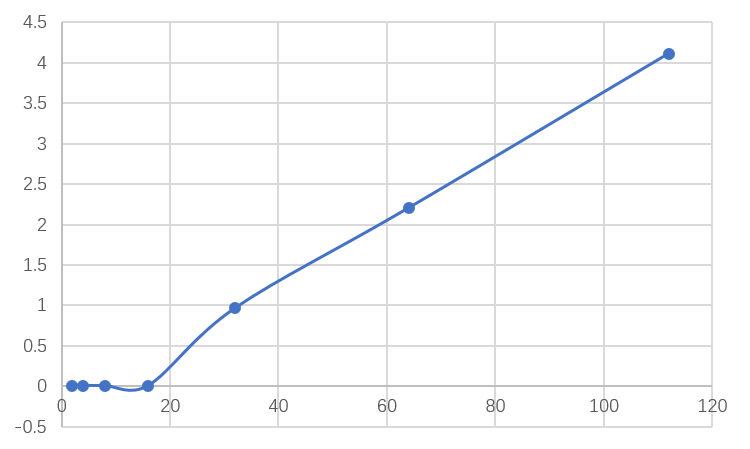
\includegraphics[width=0.4\textwidth]{14time.png}
  \label{fig:14time}}
  \subfigure[$n=2^{26}$时间变化]{
  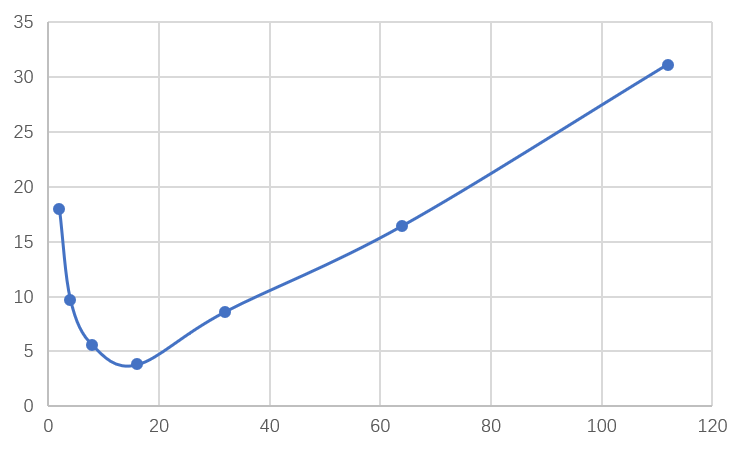
\includegraphics[width=0.4\textwidth]{26time.png}
  \label{fig:26time}}
\end{figure}

\par 加速比如\tabref{tab:speedup}。在元素个数不变的情况下,加速比的变化与并行运行时间变化相同;
在核数不变时,随着问题规模的扩大,加速比先上升后下降,\figref{fig:speedup1}和\figref{fig:speedup2}
直观地显示了这一趋势。结合加速比公式$S_p = \frac{1}{W_s+W_p / p}$,认为是当问题规模较小时,$n$的增大更充分地发挥了每个核的计算能力,使并行部分所占的比例增大;而当规模
达到一定程度,超过每个核的计算能力,继续增大$n$就没法继续获得加速了。就像一个人1小时能做10道题,而现在
只有3道题给他做,那这1小时他的速度就是3道题/h,而如果有8道题给他,他的速度就是8道题/h,但是要是给他20道题,
他的速度也只能是10道题/h。
\begin{table}[!htbp]
    \centering
    \begin{tabular}{c|ccccccc}
        \toprule
        & 2 & 4 & 8 & 16 & 32 & 64 & 112\\
        \hline
        10 & 1.2 & 1.5 & 0.75 & 0.352941176 & 0.007100592 & 0.003460208 & 0.001409774\\
        14 & 1.637931034 & 2.794117647 & 3.653846154 & 2.714285714 & 0.00987834 & 0.004318574 & 0.002311098\\
        18 & 1.789473684 & 2.876923077 & 3.826086957 & 6.393162393 & 0.145922747 & 0.07847663 & 0.032625289\\
        22 & 1.738313556 & 2.849963154 & 4.54453584 & 6.390284204 & 1.171726353 & 0.694601099 & 0.377035116\\
        26 & 1.777969306 & 3.290489226 & 5.724951658 & 8.381828667 & 3.700510375 & 1.944359988 & 1.027342244\\
        30 & 1.752720954 & 3.223312402 & 5.287014898 & 7.915926584 & 5.153370384 & 2.76478792 & 1.491955156\\
        31 & 1.749396373 & 3.225906655 & 5.282075192 & 7.98487858 & 5.226252883 & 3.11456563 & 1.5478438\\
        32 & 1.740709578 & 3.240019315 & 5.281116382 & 7.916201652 & 5.162403826 & 3.161138346 & 1.631572029        \\
        \bottomrule
    \end{tabular}
    \caption{加速比} \label{tab:speedup}
\end{table}

\begin{figure}[H]
    \centering
    \subfigure[加速比1]{
    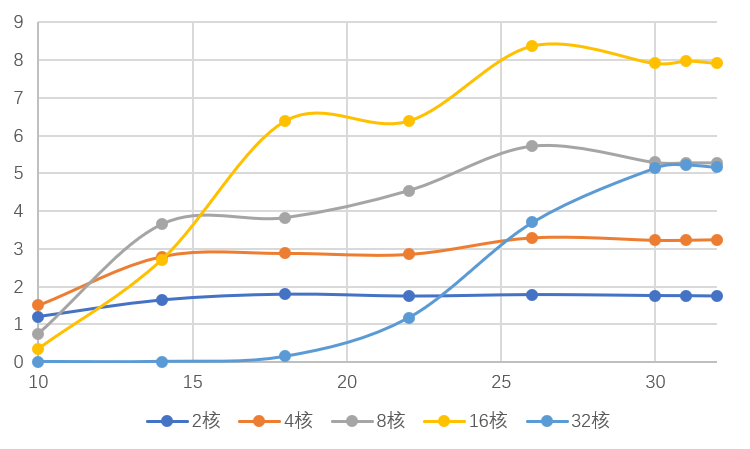
\includegraphics[width=0.4\textwidth]{speedup1.png}
    \label{fig:speedup1}}
    \subfigure[加速比2]{
    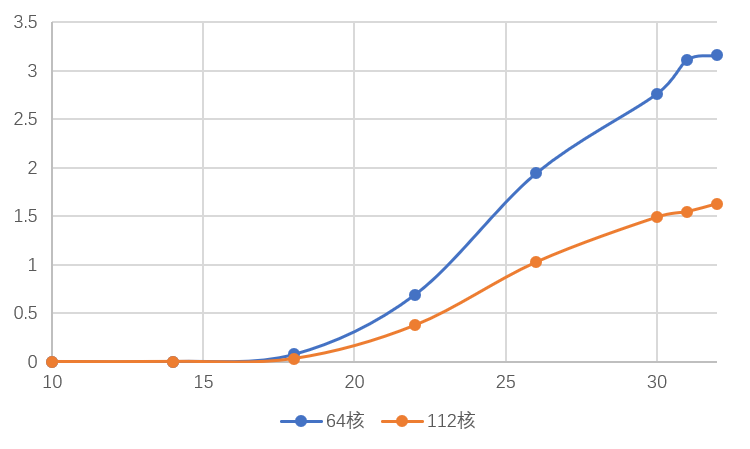
\includegraphics[width=0.4\textwidth]{speedup2.png}
    \label{fig:speedup2}}
\end{figure}

\par 在问题规模一定时,效率随着核数的增加而降低;核数一定时,效率与加速比的变化趋势一致,先升后降。
\begin{table}[!htbp]
    \centering
    \begin{tabular}{c|ccccccc}
        \toprule
        & 2 & 4 & 8 & 16 & 32 & 64 & 112\\
        \hline
        10 & 60 & 37.5 & 9.375 & 2.205882353 & 0.022189349 & 0.005406574 & 0.001258727\\
        14 & 81.89655172 & 69.85294118 & 45.67307692 & 16.96428571 & 0.030869814 & 0.006747773 & 0.00206348\\
        18 & 89.47368421 & 71.92307692 & 47.82608696 & 39.95726496 & 0.456008584 & 0.122619735 & 0.029129722\\
        22 & 86.91567781 & 71.24907885 & 56.806698 & 39.93927627 & 3.661644852 & 1.085314217 & 0.336638497\\
        26 & 88.8984653 & 82.26223064 & 71.56189572 & 52.38642917 & 11.56409492 & 3.038062481 & 0.917269861\\
        30 & 87.63604768 & 80.58281005 & 66.08768622 & 49.47454115 & 16.10428245 & 4.319981124 & 1.332102818\\
        31 & 87.46981863 & 80.64766638 & 66.0259399 & 49.90549113 & 16.33204026 & 4.866508797 & 1.382003393\\
        32 & 87.03547889 & 81.00048288 & 66.01395477 & 49.47626032 & 16.13251196 & 4.939278666 & 1.456760741\\
        \bottomrule
    \end{tabular}
    \caption{效率} \label{tab:speedup}
\end{table}

\end{document}
